% QUEST-KG architecture figure (TikZ, vector). Drop into the main paper or compile standalone.
% Three-stage pipeline: Retrieval -> Evidential MP -> Neuro-Symbolic + Abstention.

\documentclass[border=4pt]{standalone}
\usepackage{tikz}
\usetikzlibrary{positioning, shapes.geometric, arrows.meta, fit, backgrounds, calc}

\begin{document}
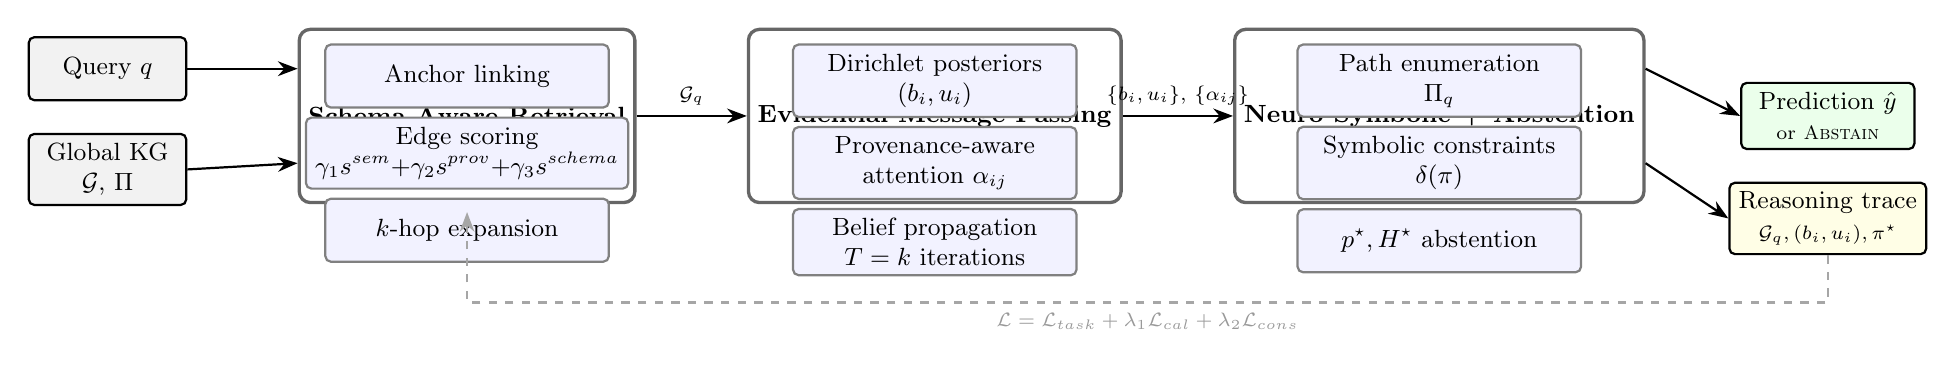
\begin{tikzpicture}[
  font=\small,
  node distance=8mm and 8mm,
  stage/.style={
    rectangle, rounded corners=4pt, draw=black!60, very thick,
    minimum width=42mm, minimum height=22mm, align=center, fill=white
  },
  module/.style={
    rectangle, rounded corners=2pt, draw=black!50,
    minimum width=36mm, minimum height=8mm, align=center, fill=blue!5
  },
  legend/.style={font=\scriptsize\itshape, align=left},
  ->, >={Stealth[length=2.5mm]},
  thick
]

% Inputs at left
\node[draw, rounded corners=2pt, fill=gray!10, minimum width=20mm, minimum height=8mm, align=center]
  (query) {Query $q$};
\node[draw, rounded corners=2pt, fill=gray!10, minimum width=20mm, minimum height=8mm,
      below=4mm of query, align=center]
  (kg) {Global KG\\ $\mathcal{G},\,\Pi$};

% Stage 1: Retrieval
\node[stage, right=14mm of query.east, anchor=west, yshift=-6mm] (s1)
  {\textbf{Schema-Aware Retrieval}};
\node[module, below=2mm of s1.north, anchor=north] (m11) {Anchor linking};
\node[module, below=1mm of m11] (m12) {Edge scoring \\ $\gamma_1 s^{\text{sem}}{+}\gamma_2 s^{\text{prov}}{+}\gamma_3 s^{\text{schema}}$};
\node[module, below=1mm of m12] (m13) {$k$-hop expansion};

% Stage 2: Evidential MP
\node[stage, right=14mm of s1] (s2)
  {\textbf{Evidential Message Passing}};
\node[module, below=2mm of s2.north, anchor=north] (m21) {Dirichlet posteriors \\ $(b_i, u_i)$};
\node[module, below=1mm of m21] (m22) {Provenance-aware \\ attention $\alpha_{ij}$};
\node[module, below=1mm of m22] (m23) {Belief propagation \\ $T = k$ iterations};

% Stage 3: NS reasoning + abstention
\node[stage, right=14mm of s2] (s3)
  {\textbf{Neuro-Symbolic + Abstention}};
\node[module, below=2mm of s3.north, anchor=north] (m31) {Path enumeration \\ $\Pi_q$};
\node[module, below=1mm of m31] (m32) {Symbolic constraints \\ $\delta(\pi)$};
\node[module, below=1mm of m32] (m33) {$p^\star, H^\star$ abstention};

% Output at right
\node[draw, rounded corners=2pt, fill=green!8, minimum width=22mm, minimum height=8mm,
      right=12mm of s3.east, align=center] (out)
  {Prediction $\hat{y}$ \\ {\scriptsize or \textsc{Abstain}}};
\node[draw, rounded corners=2pt, fill=yellow!10, minimum width=22mm, minimum height=8mm,
      below=4mm of out, align=center] (trace)
  {Reasoning trace \\ {\scriptsize $\mathcal{G}_q, (b_i, u_i), \pi^\star$}};

% Arrows: inputs into stage 1
\draw[->] (query.east) -- ($(s1.west) + (0, 6mm)$);
\draw[->] (kg.east)    -- ($(s1.west) + (0,-6mm)$);

% Between stages
\draw[->] (s1.east) -- node[above,legend] {$\mathcal{G}_q$} (s2.west);
\draw[->] (s2.east) -- node[above,legend] {$\{b_i, u_i\},\,\{\alpha_{ij}\}$} (s3.west);

% Outputs
\draw[->] ($(s3.east) + (0, 6mm)$) -- (out.west);
\draw[->] ($(s3.east) + (0,-6mm)$) -- (trace.west);

% Training feedback loop (dashed)
\draw[->, dashed, gray!70]
  (trace.south) -- ++(0,-6mm) -| ($(s1.south)+(0,-1mm)$)
  node[pos=0.25, below, legend, text=gray!80] {$\mathcal{L} = \mathcal{L}_{\text{task}} + \lambda_1 \mathcal{L}_{\text{cal}} + \lambda_2 \mathcal{L}_{\text{cons}}$};

\end{tikzpicture}
\end{document}
